\chapter{Custom Screen Printing Setup}\label{app:screen_printing}

\begin{appbox}
	Back to Section~\ref{subsect:thin_film:experimental:doctor_screen}\hfill \hyperref[chapter:toc]{Main Table Of Content (TOC)}
\end{appbox}

\begin{figure}
	\centering
	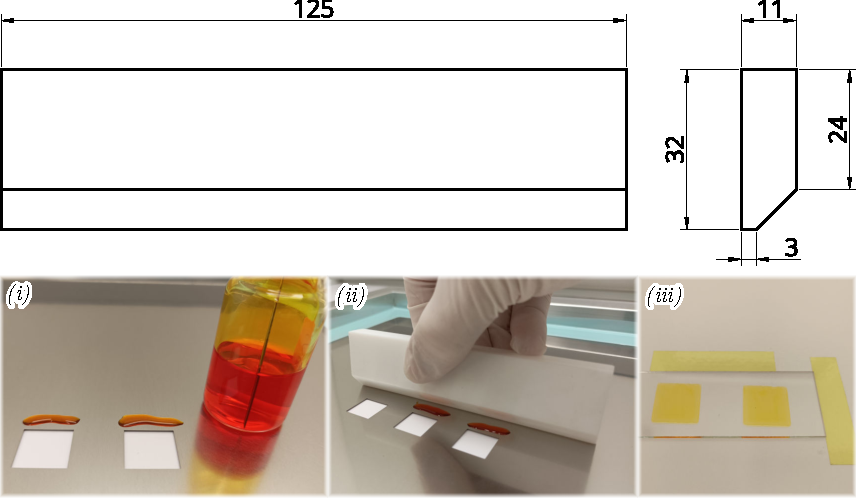
\includegraphics{3_back_matter/figures/cale_ptfe_comp.pdf}
	\caption[Custom screen printing doctor blade and setup.]{\textbf{Top:} mechanical drawing of the \gls{ptfe} doctor blade used for screen printing. \textbf{Bottom:} screen printing process. \textit{(i)}, a standard 100~\textmu{}m thick \gls{smd} stencil is positioned on top of a microscope glass slide and some amount of solution (here \gls{rudpp} and \gls{pan} in \gls{dmf}) is deposited next to the stencil's openings. \textit{(ii)}, the \gls{ptfe} doctor blade is then scraped across the surface of the stencil in a single continuous motion, spreading the solution evenly on the glass substrate. \textit{(iii)}, the resulting liquid thin-films after the stencil is removed.\\\textbf{Disclaimer:} contrary to most other aspects of this doctoral work, the blade dimensions, the scraping speed, and the overall screen printing process were not particularly fine-tuned. It yielded results at least as good as using a dedicated doctor blade setup (K Control Coater, Erichsen) while being much easier to work with, mainly due to faster cleaning times, as exposed in Section~\ref{subsect:thin_film:experimental:doctor_screen}.}
\end{figure}
